
%%%%%%%%%%%%%%%%%%%%%%%%%%%%%%%%%%%%%%%%%
% University/School Laboratory Report
% LaTeX Template
% Version 3.1 (25/3/14)
%
% This template has been downloaded from:
% http://www.LaTeXTemplates.com
%
% Original author:
% Linux and Unix Users Group at Virginia Tech Wiki 
% (https://vtluug.org/wiki/Example_LaTeX_chem_lab_report)
%
% License:
% CC BY-NC-SA 3.0 (http://creativecommons.org/licenses/by-nc-sa/3.0/)
%
%%%%%%%%%%%%%%%%%%%%%%%%%%%%%%%%%%%%%%%%%

%----------------------------------------------------------------------------------------
%	PACKAGES AND DOCUMENT CONFIGURATIONS
%----------------------------------------------------------------------------------------

\documentclass{article}

\usepackage{physics}
\usepackage{siunitx} % Provides the \SI{}{} and \si{} command for typesetting SI units
\usepackage{graphicx} % Required for the inclusion of images
\usepackage{natbib} % Required to change bibliography style to APA
\usepackage{amsmath} % Required for some math elements 
\usepackage{subcaption}
\usepackage{caption}
\usepackage{mathtools}
\usepackage{listings}
\usepackage{placeins}

\setlength\parindent{0pt} % Removes all indentation from paragraphs

\renewcommand{\labelenumi}{\alph{enumi}.} % Make numbering in the enumerate environment by letter rather than number (e.g. section 6)

%\usepackage{times} % Uncomment to use the Times New Roman font

%----------------------------------------------------------------------------------------
%	DOCUMENT INFORMATION
%----------------------------------------------------------------------------------------

\title{Vibrational effects on molecular spectra} % Title

\author{Arttu Hyv\"onen} % Author name

\date{\today} % Date for the report

\begin{document}

\maketitle % Insert the title, author and date

\begin{center}
\begin{tabular}{l l}
 \\ 
Instructors:    & Marc Dvorak \\
                & Patrick Rinke 
\end{tabular}
~\\~\\
Aalto University, Department of Applied Physics
\end{center}


%----------------------------------------------------------------------------------------
%	SECTION 1
%----------------------------------------------------------------------------------------
~\\
\section{Objective}

Objective for this project was to produce ionization spectrum with vibrations for complex molecule using computational methods and more specifically FHI-AIMS.


%----------------------------------------------------------------------------------------
%	SECTION 2
%----------------------------------------------------------------------------------------
~\\
\section{Methods}

There's three main steps in finding the vibrational spectra: finding equilibrium geometry, vibrational frequencies and calculating overlap integrals.

\subsection{Equilibrium geometry}

To find equilibrium geometry molecules were relaxed with FHI-AIMS using keyword \lstinline{relax_geometry}. Calculations were also done for molecules in exited electronic state. To accomplish this keyword \lstinline{force_occupation_projector} was used. Really tight second tier settings were used for atoms and PBE was used as a functional.

\subsection{Vibrational frequencies}

Vibrational frequencies and corresponding reduced masses were calculated with script provided in FHI-AIMS utilities. Previously found equilibrium geometry was used as a base geometry, but otherwise input files were unchanged.

\subsection{Overlap integrals}

Calculating the overlap integral follows closely methods used by Gallandi and K\"orzd\"orfer \cite{gall2015}. If potential surfaces are approximated as harmonic potentials, integral can be calculated in form
\begin{align}
    & \mathrm{FCI}(n_i, n'_i)^2 = e^{-S_i}S_i^{n'_i-n_I} \frac{n_i!}{n'_i!} \left[L_{n_i}^{n'_i-n_i}(S_i)\right]^2 \nonumber \\
    & S_i = \delta_i^2 \mu_i f_i/2\hbar \nonumber
\end{align}
where $\mu_i$ is reduced mass corresponding to frequency $f_i$. There is two values for each $\mu_i$ and $f_i$, one for the initial state and one for the final state. Values for the final state, which in this case is the exited electronic state, were used. $\delta_i$ is obtained by first finding the separation between initial and final geometry, then transforming that separation from cartesian coordinates to vibrational normal mode coordinates, and then taking the component $i$. $n$ and $n'$ are lists of vibrational quantum numbers for initial and final state. Every mode for which $S_i < S_min$ is dropped out as irrelevant. Intensity of delta peaks can then be calculated with equation
\begin{align}
    \mathrm{I}(n, n') &= \prod_{i=0}^p \;
    {\overbrace{\textstyle \mathrm{FCI}(n_i, n'_i)^2}^{\mathclap{\text{Overlap integral}}}} \;
    {\underbrace{\textstyle \exp\left( \frac{-\hbar n_i f_i}{k_B T} \right)}_{\mathclap{\text{Temperature term}}}} \nonumber 
\end{align}
where $p$ is a set of relevant modes. Intensity calculation is then repeated for all combinations of $n$ and $n'$ where $\sum_{i=0}^p n_i < A$ and $\sum_{i=0}^p n'_i < B$. With intensities calculated, peak energies are obtained by adding vibrational energy to the peak without vibrations. Vibrational energy can be calculated with $$E_{vib} = \sum_{i=0}^p \left[h f_i(n_i + 1/2)\right]$$ 
The peaks without vibrations were calculated using $G_0W_0$. In the case of benzene there's also peaks calculated with DCI. All the vibrational calculations and by extension vibrational energies used only PBE.

%----------------------------------------------------------------------------------------
%	SECTION 3
%----------------------------------------------------------------------------------------
~\\
\section{Results}

Usually every electronic transition has around $10-100$ vibrational peaks that have a relative intensity of $0.001$ or more, when the largest peak is in the range $0.5-1.0$. As an example in the Table 1 there's vibrational peaks for one of the benzenes ionizations and in the Figure 1 same peaks plotted.

\begin{table}[h!]
    \centering
    \begin{tabular}{c c c}
        \textbf{Intensity} & \textbf{Energy $\textbf{G}_0\textbf{W}_0$@PBE (eV)} & \textbf{Energy DCI (eV)} \\ \hline
        0.7107 & 11.635 & 12.318 \\ % \hline 
        0.2389 & 11.767 & 12.450 \\ % \hline 
        0.0402 & 11.899 & 12.582 \\ % \hline 
        0.0045 & 12.031 & 12.714 \\ % \hline 
        0.0038 & 12.026 & 12.709 \\ % \hline 
        0.0013 & 12.158 & 12.841 \\ % \hline 
        0.0012 & 11.503 & 12.186 \\ % \hline 
        0.0016 & 11.635 & 12.318 \\ % \hline 
        0.0017 & 11.767 & 12.450 \\  \hline 
    \end{tabular}
    \caption{Relative intensities and positions for the vibrational peaks of the fifth ionization transition of benzene. Zero-zero transition energies calculated with either $\text{G}_0\text{W}_0$@PBE or DCI and vibrational energies with PBE.}
\end{table}
\FloatBarrier

\begin{figure}[h!]
    \centering
    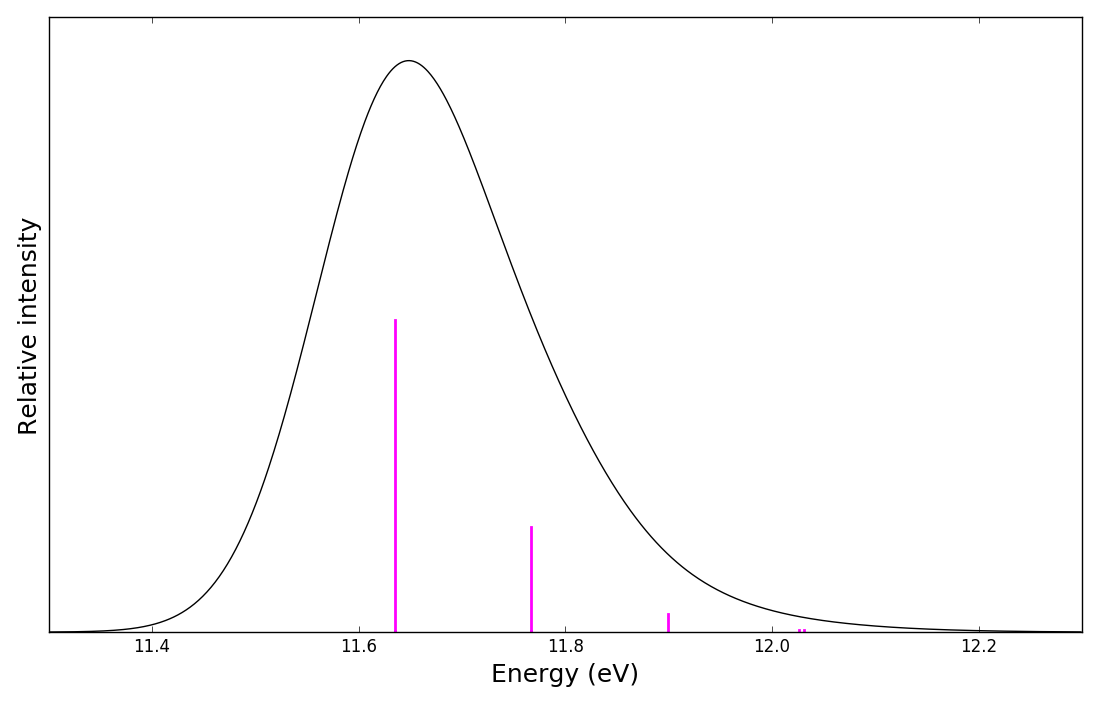
\includegraphics[width=\textwidth]{4th_peak.png}
    \caption{Fifth ionization peak of benzene with gaussian broadening of 0.08 eV. 0-0 peak position with $\text{G}_0\text{W}_0$@PBE.}
\end{figure}


In the Figure 2 is the ionization spectra the of benzene with ten first transitions. From top to bottom, experimental, $\text{G}_0\text{W}_0$@PBE without vibrations, and $\text{G}_0\text{W}_0$@PBE with vibrations. In the Figure 3 is the same spectra, but with DCI values and only fife first transitions.

\begin{figure}[h!]
    \centering
    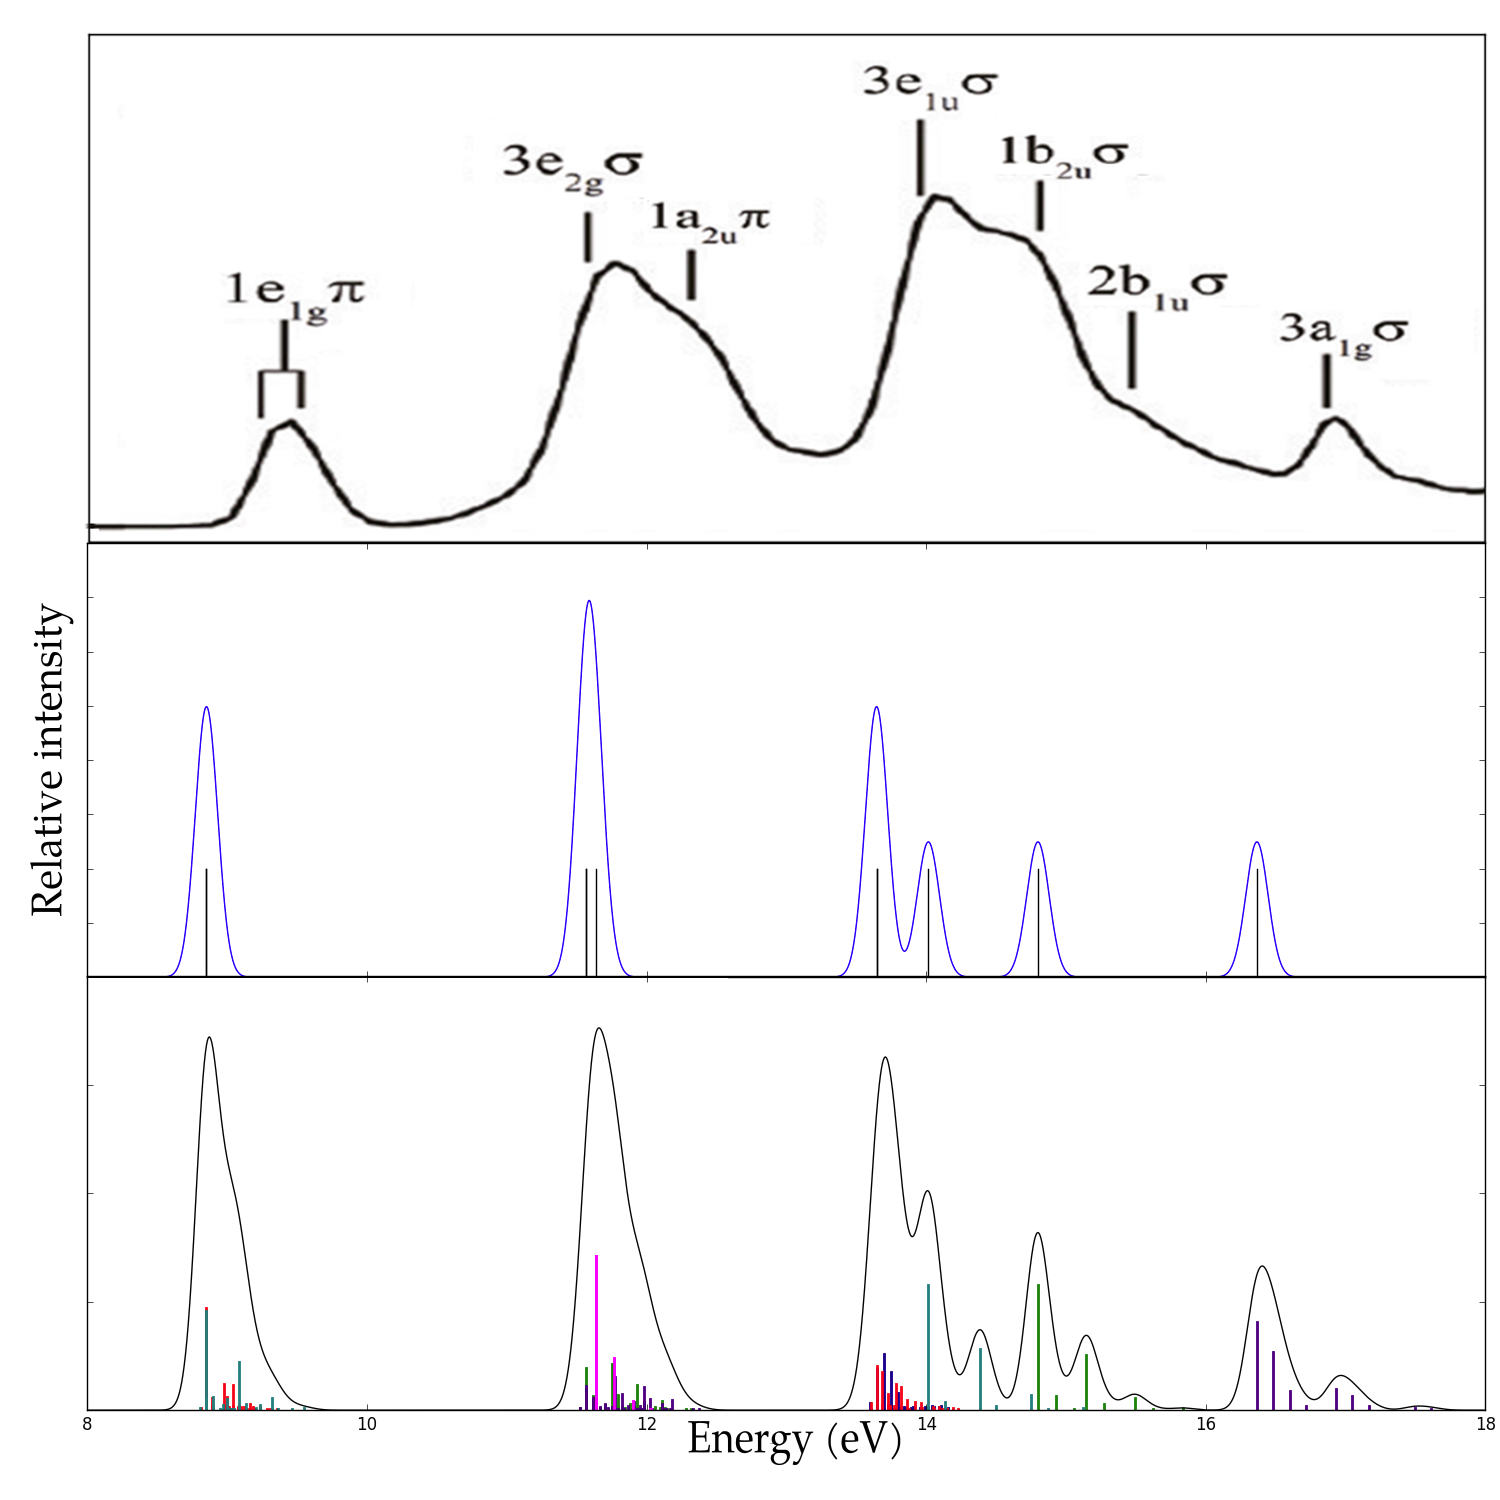
\includegraphics[width=0.8\textwidth]{GW_experiment.png}
    \caption{Ionization spectra of benzene with gaussian broadening of 0.08 eV. 0-0 peak position with $\text{G}_0\text{W}_0$@PBE. Experimental spectrum is taken from \cite{liu2011}}
\end{figure}

\begin{figure}[h!]
    \centering
    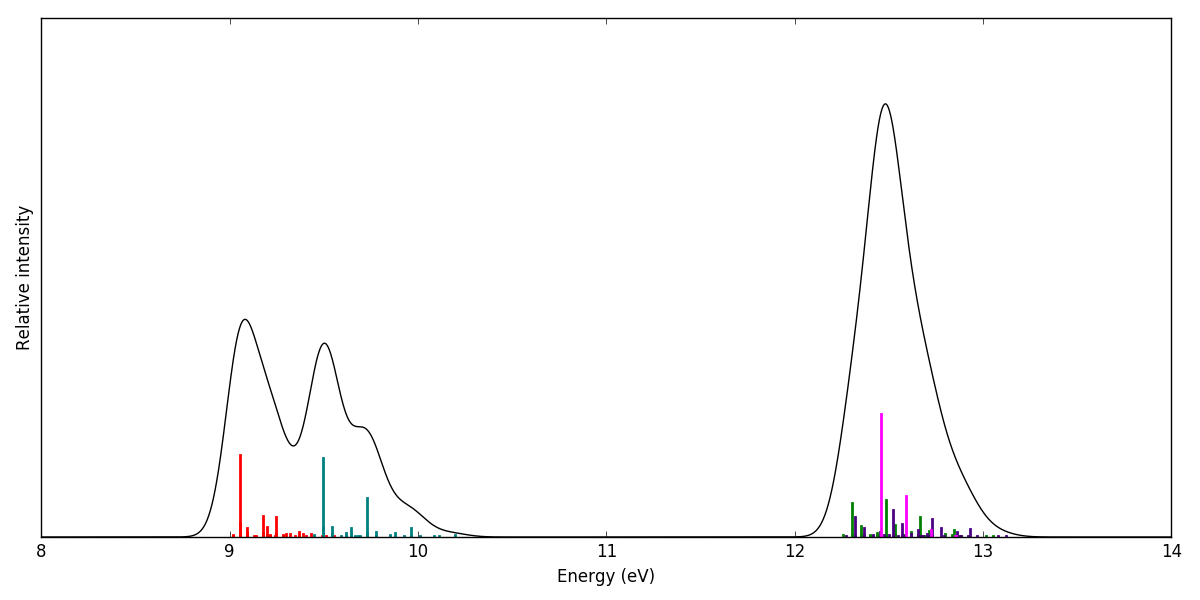
\includegraphics[width=0.8\textwidth]{DCI.png}
    \caption{Ionization spectra of benzene with gaussian broadening of 0.08 eV. 0-0 peak position with DCI.}
\end{figure}

\FloatBarrier

~\\~\\
%----------------------------------------------------------------------------------------
%	BIBLIOGRAPHY
%----------------------------------------------------------------------------------------

\bibliographystyle{plain}

\bibliography{sample}

%----------------------------------------------------------------------------------------


\end{document}
